\section{Computational discussions}

During the project we realized we had to do some computational optimization because the problems we work can generate huge matrices. Some interesting tidbits found by running and timing matlab using the profiler we have seen that:


\begin{figure}[ht]
        \centering
        \begin{subfigure}[b]{0.45 \textwidth}
                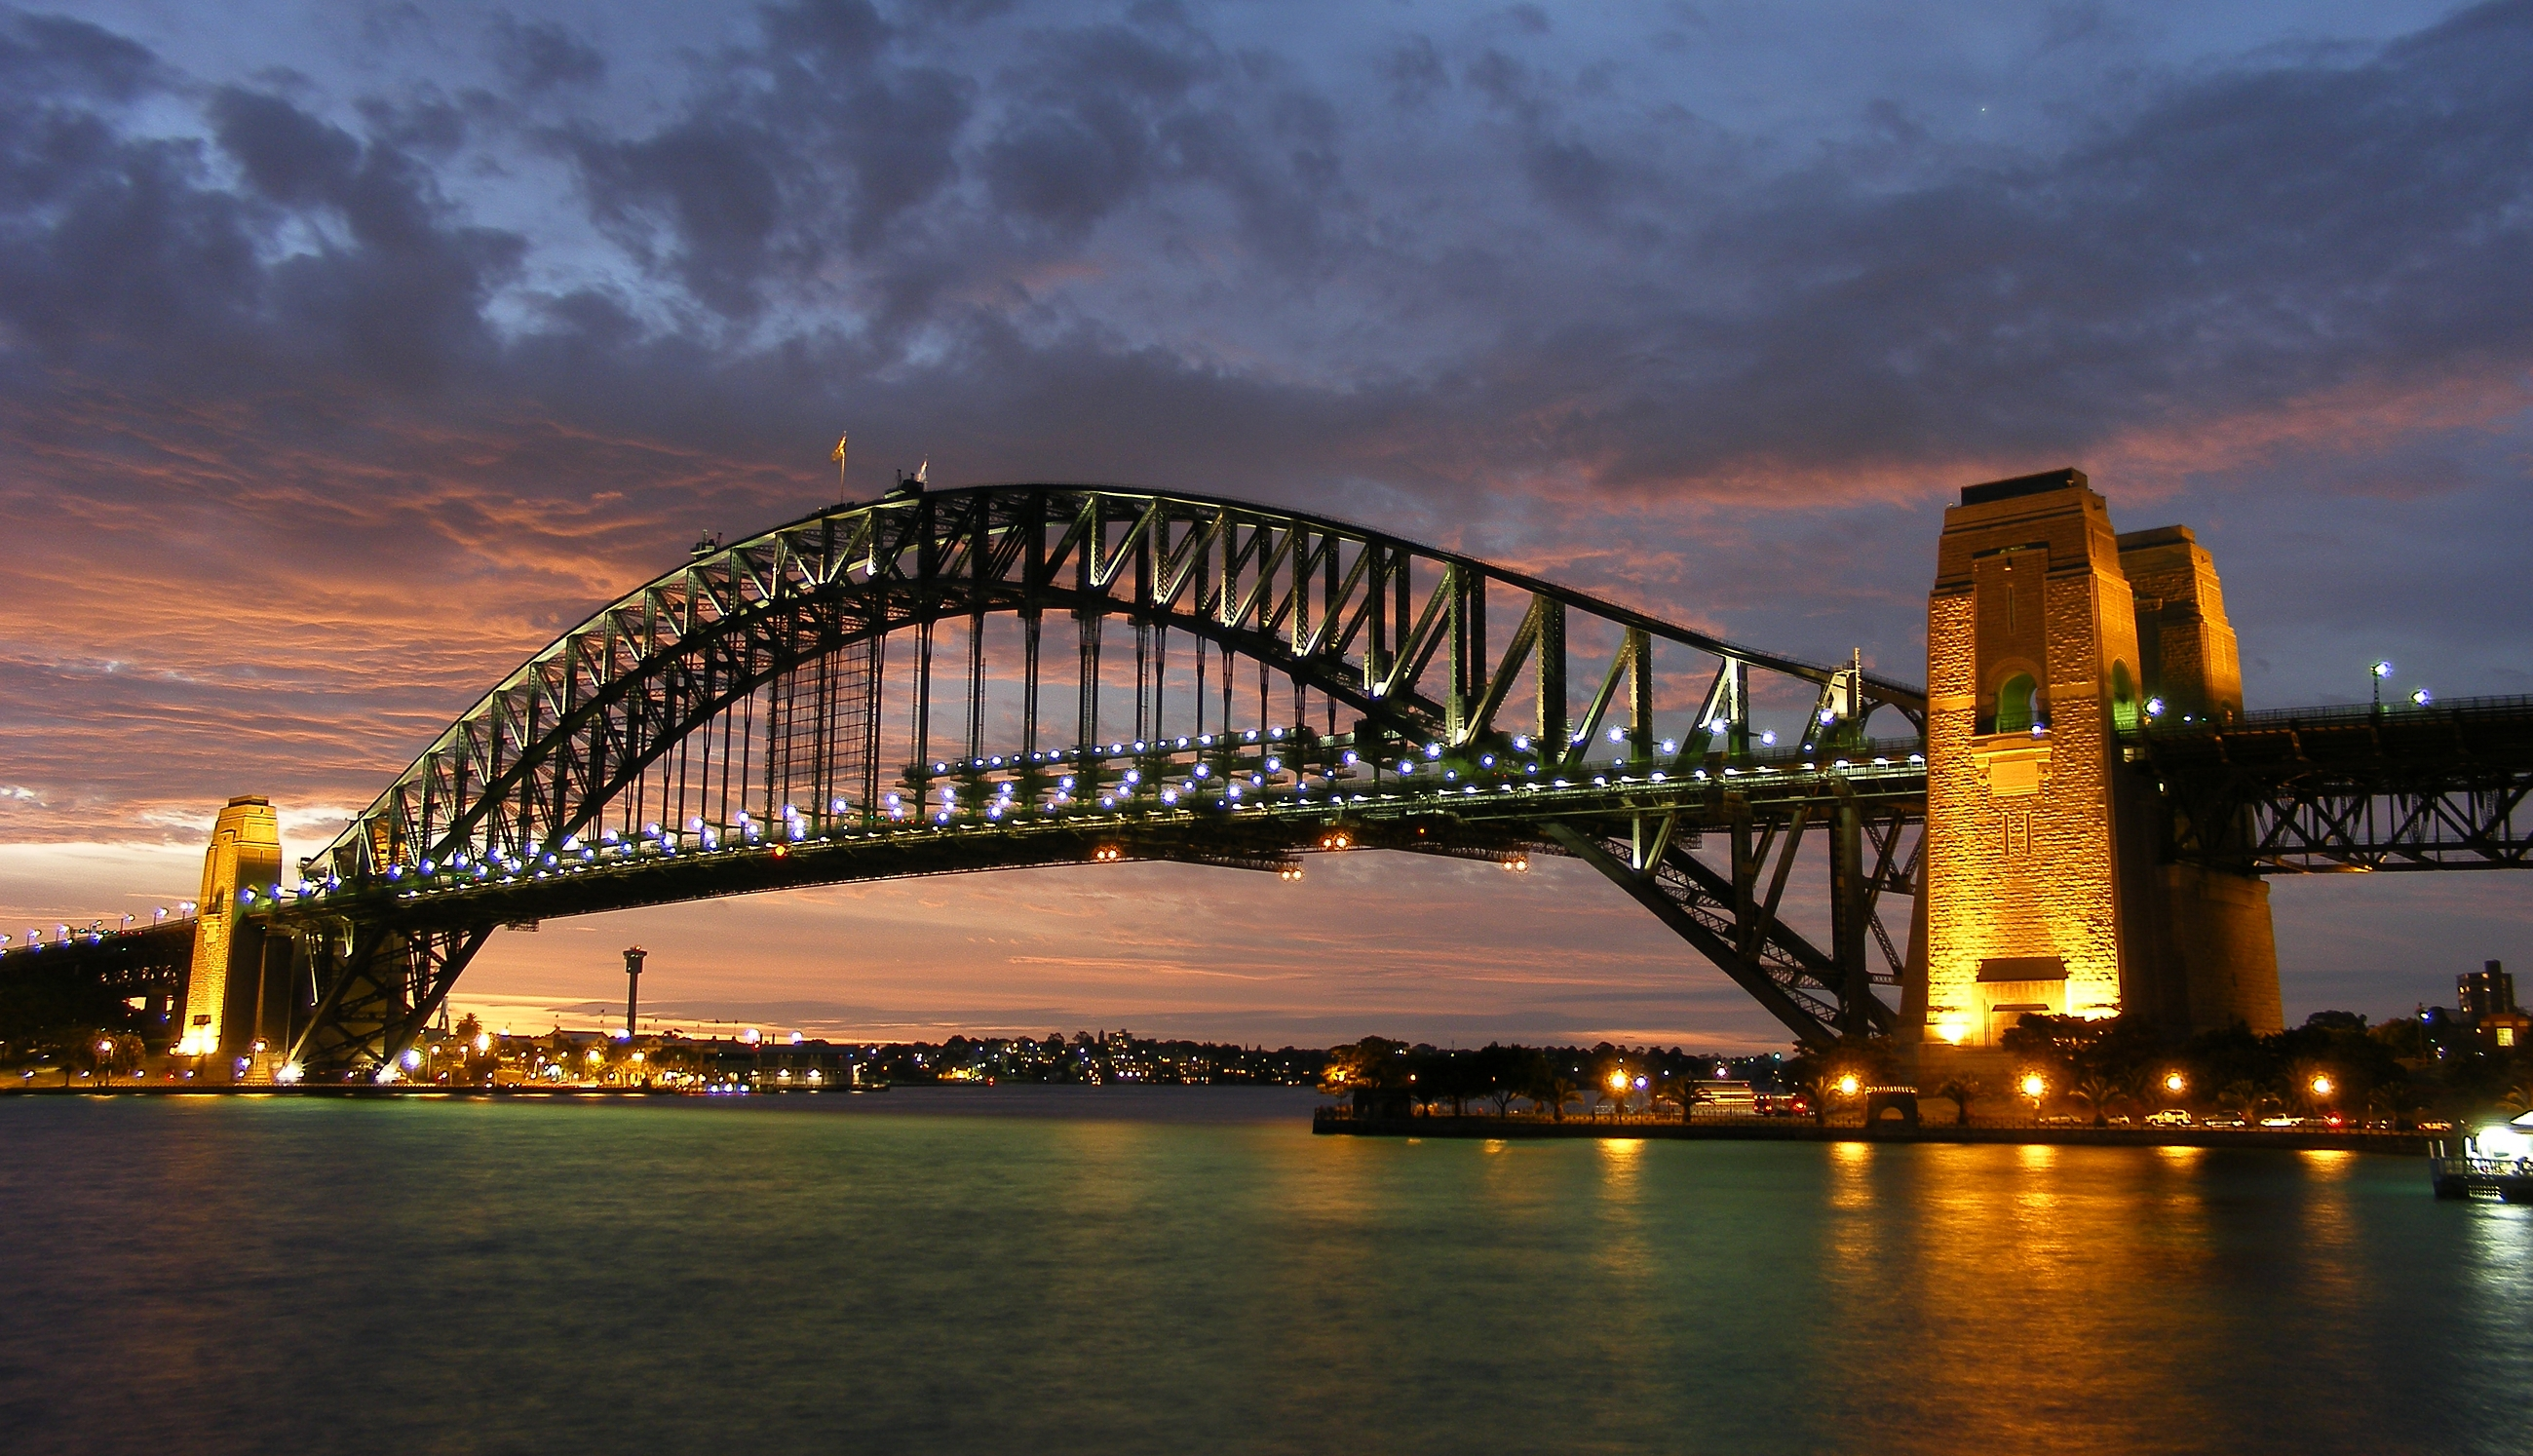
\includegraphics[width=\textwidth]{Sydney_pic}
                \caption{The Sydney harbour bridge}
        \end{subfigure}
        ~
        \begin{subfigure}[b]{0.45 \textwidth}
                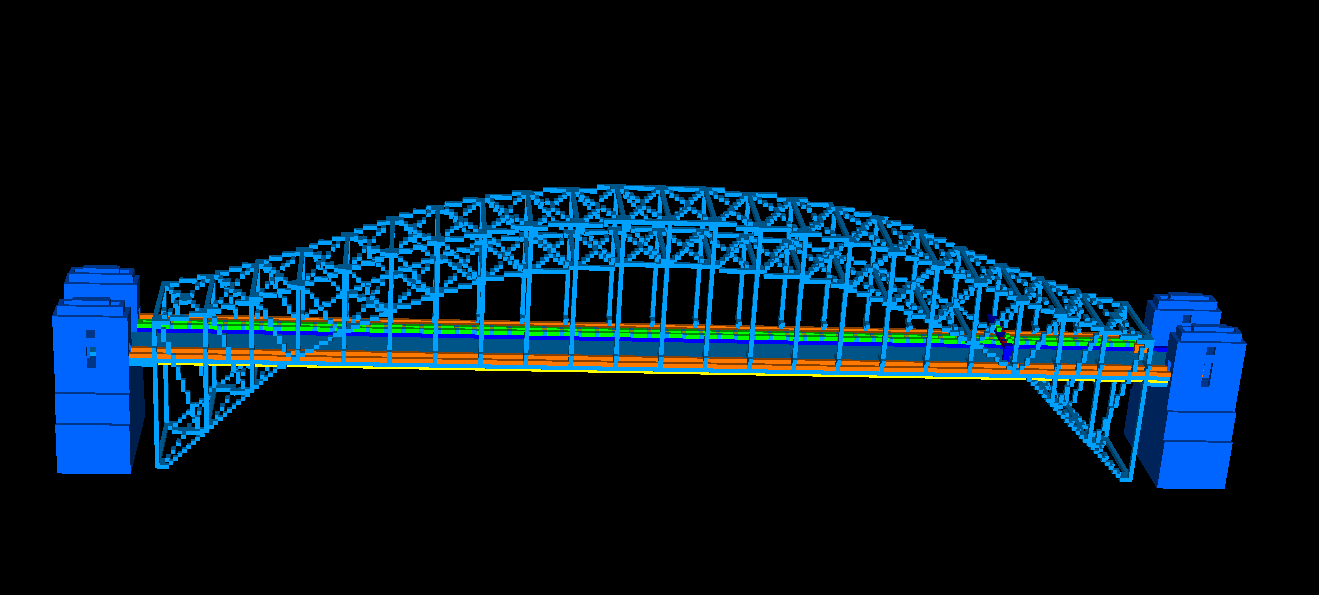
\includegraphics[width=\textwidth]{sydneyBridge}
                \caption{Minecraft model of the Sydney harbour bridge, downloaded from }
        \end{subfigure}
        \caption{The Sydney harbour bridge. This bridge proved to be too computationally intensive to be solved, even when run in parallel. There was just shy of 1 million tetrahedrons in the mesh.}
        \label{fig:sydney}
\end{figure}



\begin{itemize}
\item Sparse matrices really outperform dense matrices in the backslash operation.
\item Dense matrices really outperform sparse matrices in the assembly process of the stiffness matrix.
\item Because of the previous two points, in some cases the performance is radically improved by assembling the stiffness matrix as a dense matrix and converting it to a sparse one before we perform the backslash routine.
\item No matter how many different combinations of sparse and dense matrices we tried, you can't get around the fact that the sparse matrices require less memory, and in some of the larger problems we tried there weren't enough memory available to make a large enough dense matrix (even split upon 24 instances of matlab with a clustered matrix) We gave the Sydney harbor bridge a try (see figure \ref{fig:sydney}), but the system was too large.
\item Building of the element stiffness matrices can be run in parallel, which is really simple with the new parfor loop in matlab. The assembly process, however, cannot (as far as we can see at least). Since it's really the assembly that takes time (at least for sparse matrices), there's not really much performance improvement to get here.
\item Our bridge problem is well suited for running in parallel, since the time steps doesn’t depend on each other. (1419 seconds vs?)
\end{itemize}
